\documentclass{article}
% Choose a conveniently small page size
% PACKAGES
\usepackage[margin = 1in]{geometry}
\usepackage{amsfonts}
\usepackage{amsmath}
\usepackage{amssymb}
\usepackage{multicol}
\usepackage{graphicx}
\usepackage{float}
\usepackage{xcolor}
\usepackage{amsthm}
\usepackage{dsfont}
\usepackage{hyperref}

% MACROS
% Set Theory
\def\N{\mathbb{N}}
\def\R{\mathbb{R}}
\def\C{\mathbb{C}}
\def\Z{\mathbb{Z}}
%\def\^{\hat}
\def\-{\vec}
\def\d{\partial}
\def\!{\boldsymbol}
\def\X{\times}
%\def\-{\bar}
\def\bf{\textbf}
\def\l{\left}
\def\r{\right}
\title{Weekly Report}
\author{Damien}
\begin{document}
\maketitle
% \newpage
\section{Progress}
This week I finished replicating the results of 5.1.1 and 5.3.1 from Chen et al. Using this code gave the following tables. The exact values I am getting are different than what I see in the paper. I am achieving above third order accuracy and my errors are lower than theirs so I am happy with these results.
\subsection*{5.1.1}
\begin{figure*}[h]
    \centering
    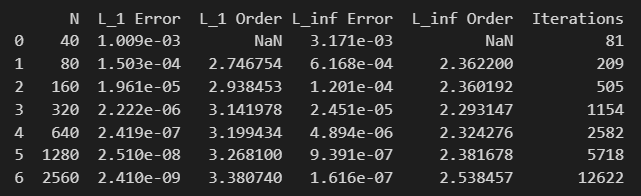
\includegraphics[width=0.5\textwidth]{imgs/5_1_1_table.png}
    \caption{This plot is an attempt to reproduce the results from Table 1 in Chen et al.}
\end{figure*}
\subsection*{5.3.1}
\begin{figure*}[h]
    \centering
    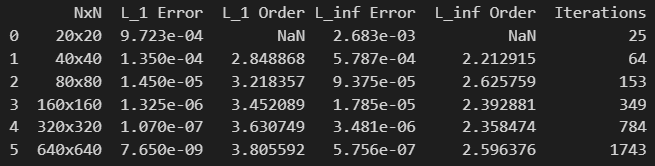
\includegraphics[width=0.5\textwidth]{imgs/5_3_1_table.png}
    \caption{This plot is an attempt to reproduce the results from Table 3 in Chen et al.}
\end{figure*}
\section{To Do}
This is everything that I have been asked to do thus far. What is the next step?
\end{document}